\documentclass[]{scrartcl}
\usepackage[turkish]{babel}
\usepackage[utf8]{inputenc}
\usepackage[T1]{fontenc}
\usepackage{graphicx}

%opening
\title{Kullanışlı Türev Alıcı İşlemsel Yükselteç}
\author{M.Zeynel Akçin 131024016 - Hüsamettin Ertürk 131024006}

\begin{document}

\maketitle

\begin{abstract}
Elektronik 1 dersi proje ödevi kapsamında verilen devrelerden beşincisi olan "Practical Differantiator" seçilmiştir. Devre hakkında bilgiler edinilmiş ve benzetimler yapılmıştır.
\end{abstract}

\section{Genel Türev Alıcı Devre ve Uygulanabilir Hali}
Elektronik devreler istenen işaretlerin yanında gürültü olarak adlandırılan işaretlerde taşıyabilmektedir. Bu gürültüler başka elektronik devrelerden kaynaklandığı gibi sistemin kendisinden de kaynaklanabilir. Bu durumda ideal olarak tasarladığımız ve bu tip gürültüleri ihmal ettiğimiz sistemleri gerçek devrelerde kullanmak beklediğimizden farklı sonuçlar elde etmemize sebep olabilir.

\begin{figure}
	\shorthandoff{=}
	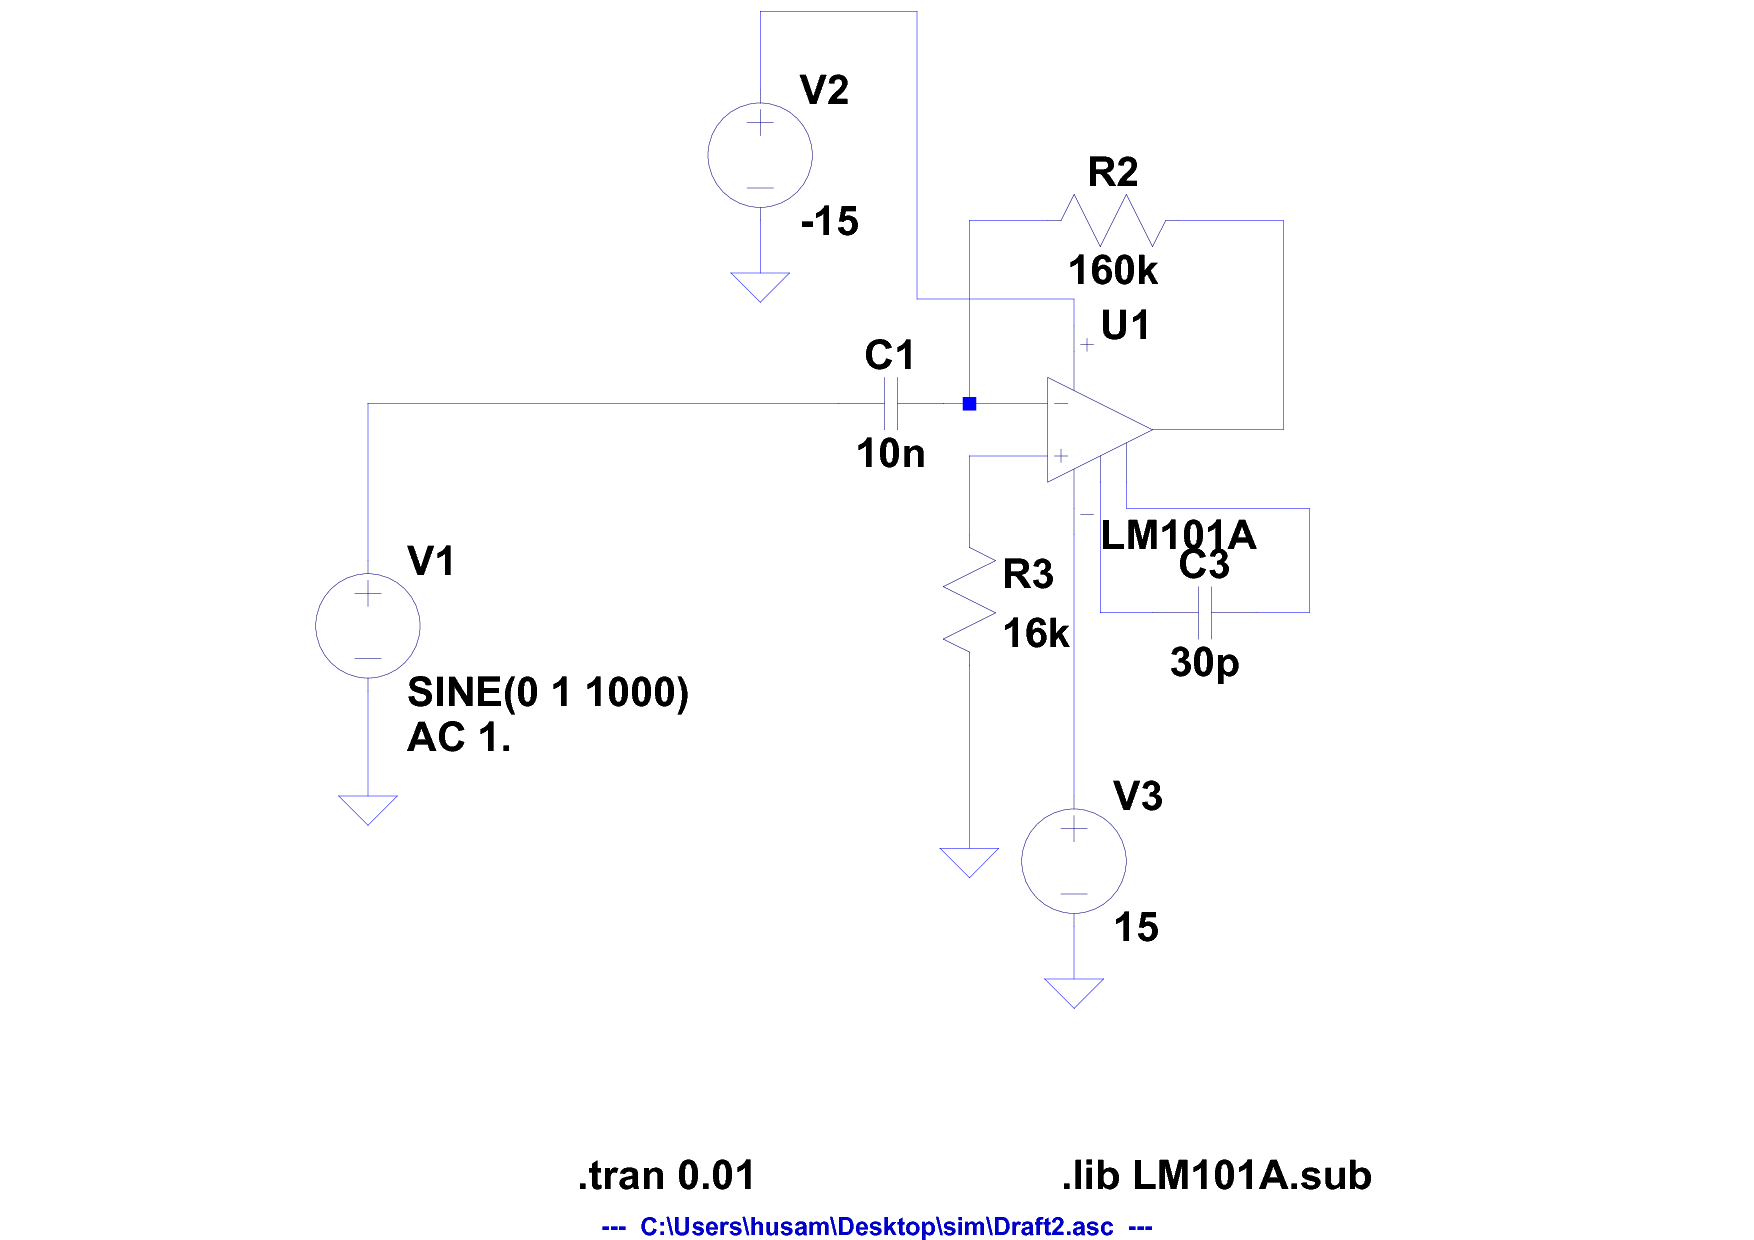
\includegraphics[width=\linewidth]{Draft4}
	\shorthandon{=}
	\caption{Genel Türev Alıcı Op-amp Devresi}
\end{figure}

Şekil 1'de görülen ideal türev alıcı devre yüksek frekanslı bir gürültüye maruz kaldığında çıkışında asıl işaretimizin türevi yerine, gürültünü katlarca yükseltilmiş halini görürüz.

Bu durumu engellemek için girişe bir direnç ve R2 direncine paralel bir kondansatör eklersek kazancı düşürür ve gürültülerin yükseltilmesini engelleriz.
\section{Benzetimler}
Şekil 2'de benzetimi yapılan uygulanabilir türev alıcı op-amp devresi görülmektedir. Devre fh 1 KHz olacak  şekilde tasarlanmıştır. fc ise 100 hz dir.  Şekil 3 ise bu devrenin 1 Khz deki giriş ve çıkış işaretleridir. Şekilde 4'de de devrenin frekans cevabı görülmektedir.

\begin{figure}
	\shorthandoff{=}
	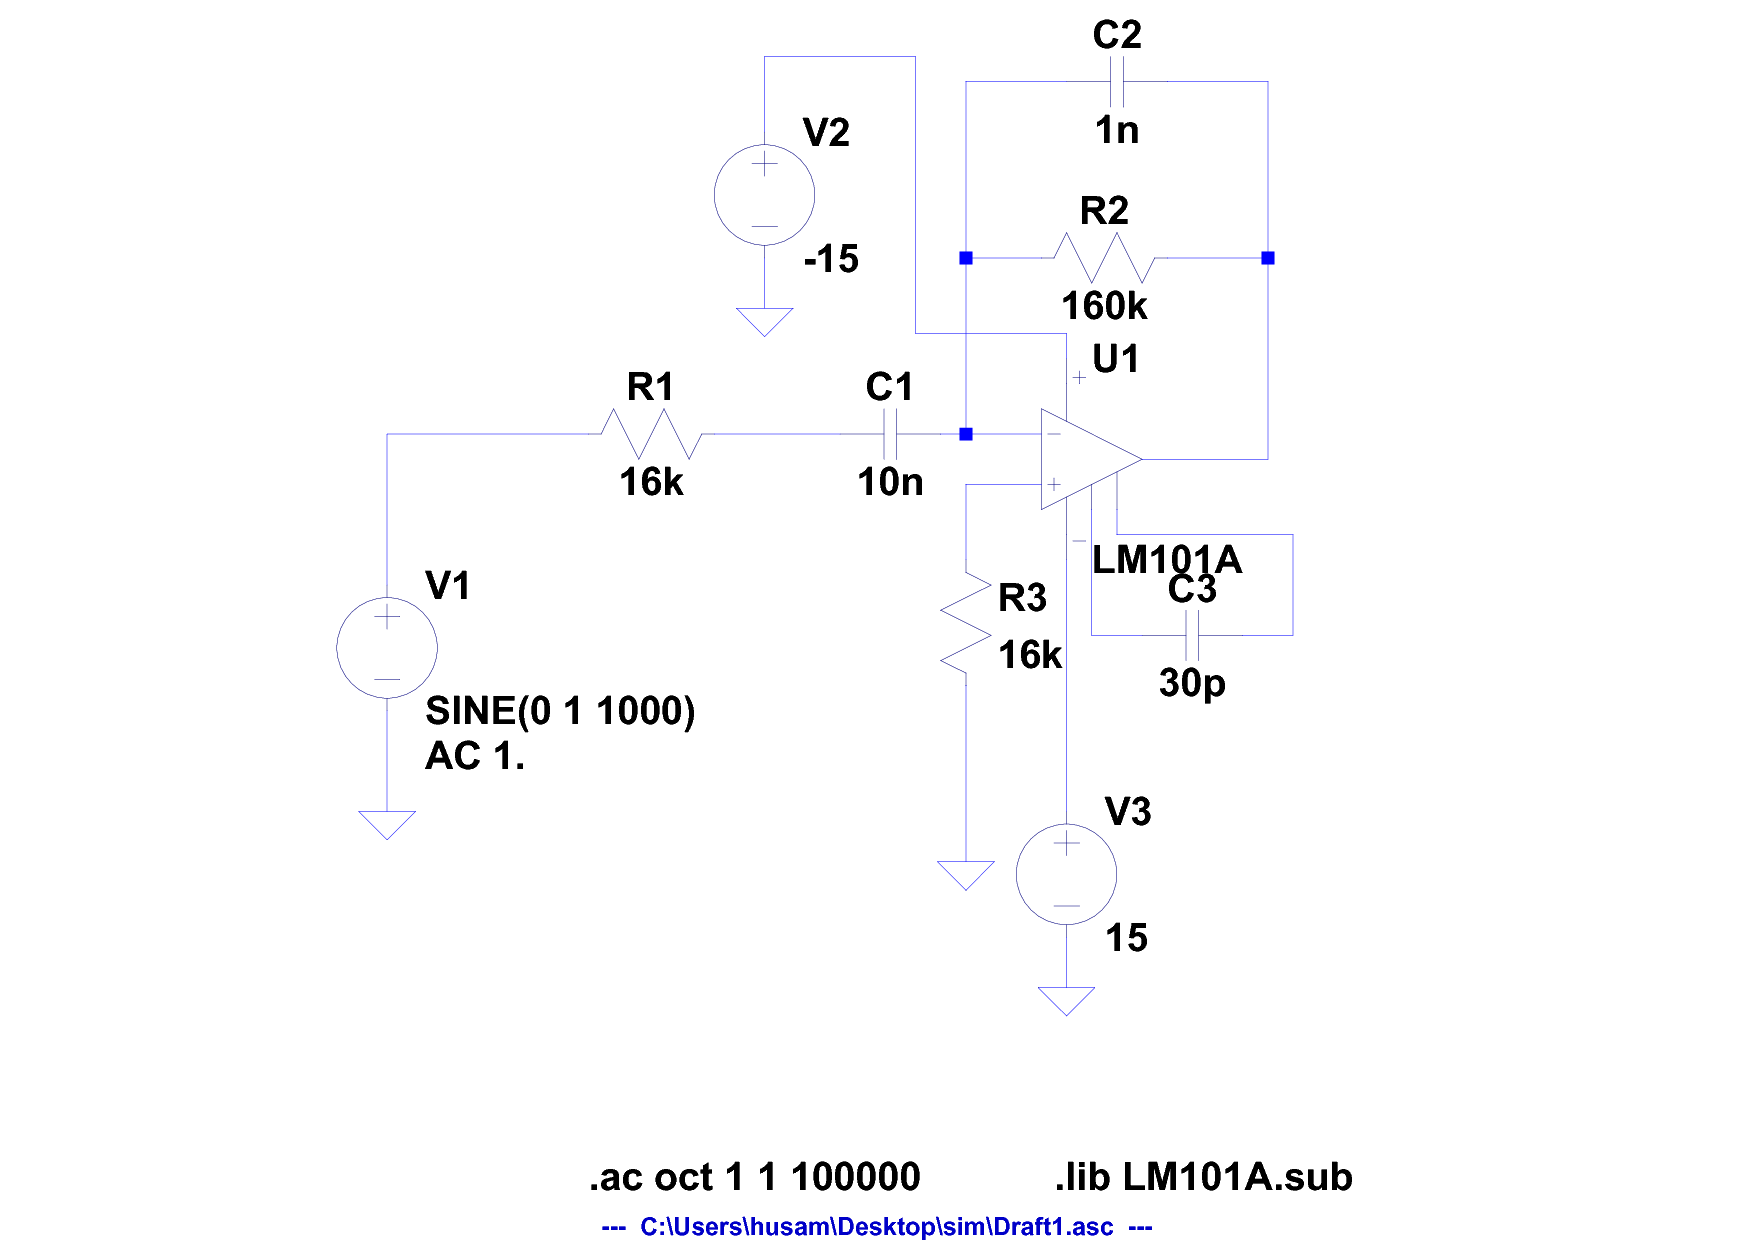
\includegraphics[width=\linewidth]{Draft3}
	\shorthandon{=}
	\caption{Uygulanabilir türev alıcı op-amp devresi}
\end{figure}

\begin{figure}
	\shorthandoff{=}
	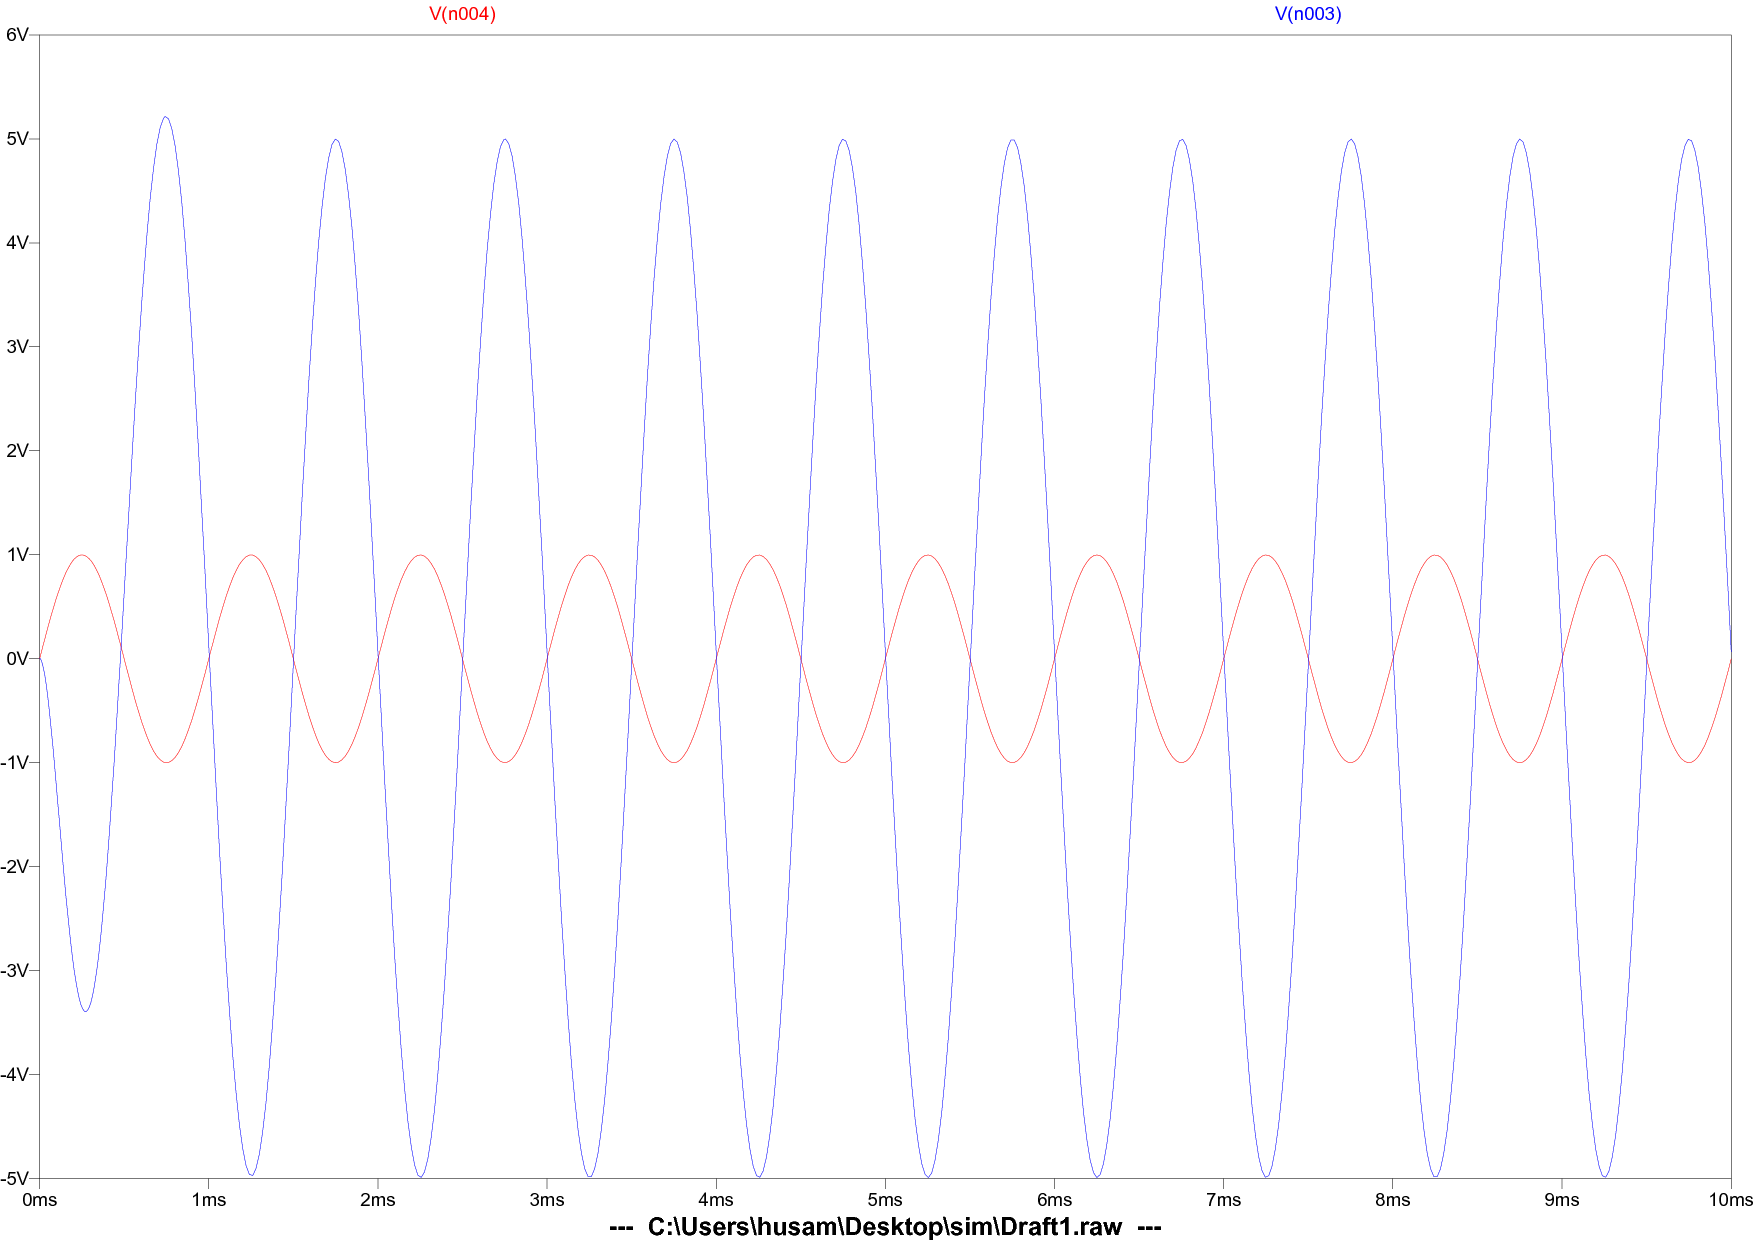
\includegraphics[width=\linewidth]{Draft1}
	\shorthandon{=}
	\caption{Devrenin 1Khz deki giriş-çıkış işaretleri}
\end{figure}

\begin{figure}
	\shorthandoff{=}
	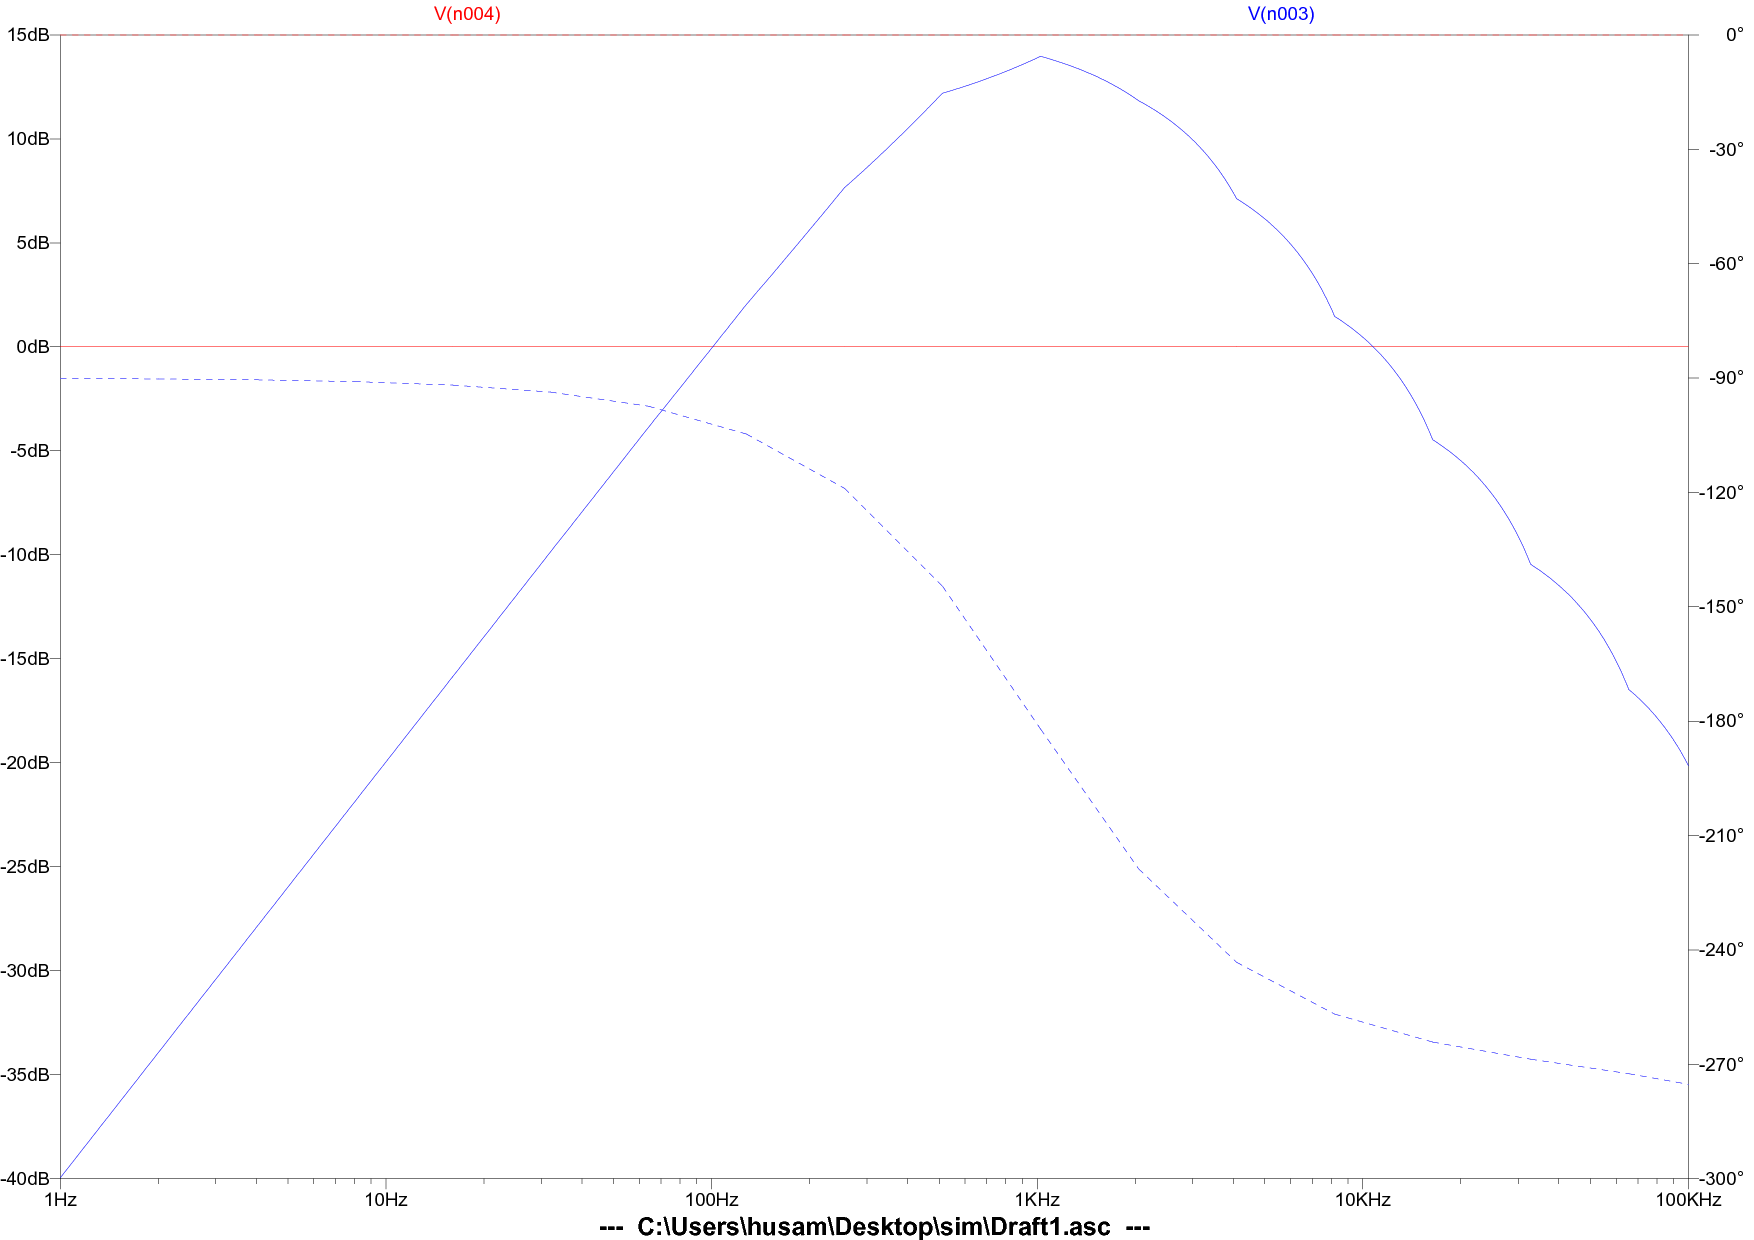
\includegraphics[width=\linewidth]{Draft2}
	\shorthandon{=}
	\caption{Devrenin frekans fevabı}
\end{figure}

\section{Kullanım Alanları}


\end{document}
